\chapter{Design}\label{design}

The following chapter will expose the design process and reasoning
behind certain design decisions made for the prototypes. It will lead
through the different prototyping stages and user testing to an
evaluation of the design, including an outlook.

The prototyping was happening in three subsequent stages. The first
stage comprised a set of pencil sketches on paper; the second prototype
was created with web technology, but fixed around a certain source code
and faked interactivity; the third prototype was implemented as a
plug-in for the Atom editor, and is able to work with any source code it
is provided.

\section{Definitions}\label{definitions}

To be able to talk about the qualitites of the concept and prototypes,
we must first define a number of terms.

\begin{description}
\item[Scope block]
In a JavaScript text file, a scope block is the textual block
representing a logical scope. For a function, which in JavaScript
creates a new scope, the scope block starts at the \texttt{function}
keyword and ends at the closing curly brace \texttt{\}} of the function
body. If, in a text editor, the cursor is placed anywhere inside this
scope block (but outside of child scopes), the scope block is called
\emph{active scope}.
\item[Current scope]
In a running JavaScript program, it is the currently executed scope.
This is a term related to the run-time rather then to author-time, and
should not be confused with \emph{active scope} described below.
\item[Active scope]
The scope which is currently in focus of editing. In relation to IDEs,
code editors and the prototypes presented in this chapter, the active
scope always describes the scope that the cursor is placed in.
\item[Local scope]
In the context of nested scopes, the local scope is the one in focus (be
it in the execution context during run-time, or the editing context
during author-time). Local scope is contrasted with non-local scope;
scopes that are logically distant from the local scope. Those may be
ancestor scopes, descendant scopes, or parallel scopes. The term is also
used to contrast \emph{global scope}.
\end{description}

\section{Sketching}\label{sketching}

One could argue that sketching is part of the earlier exploration phase,
rather than of the prototyping phase. However, next to sketching
different ideas, the author also sketched different possible
implementation for one feature that seemed valuable to the design
solution: \emph{highlighting}.

The basis for the sketches were printouts of the same source code, each
leading to a different way of highlighting.

(scans here)

\subsubsection{Active scope, inclusive}\label{active-scope-inclusive}

This sketch highlights the active scope block by applying a background
colour to it. The highlighting is \emph{inclusive}, i.e. any descendant
(inner) scopes are highlightes as well.

\subsubsection{Active scope, exclusive}\label{active-scope-exclusive}

Same as above, but descendant scope blocks are excluded from
highlighting. This way of highlighting was implemented in the static
prototype (see \ref{}).

\subsubsection{Active scope and ancestor
scopes}\label{active-scope-and-ancestor-scopes}

Next to highlighting the active scope, its ancestor scopes can also be
highlighted to emphasize nesting. To contrast the ancestor scopes from
the active scope, the highlighting would make use of different
background colours, for example different shades of grey. This way of
highlighting can be combined with both the inclusive and exclusive
approach.

\subsubsection{Scope colouring}\label{scope-colouring}

Described by Crockford \citeyear{crockford} as „context colouring“, this
way of highlighting would not apply a background colour, but instead
replace the existing forms of syntax highlighting. Thus, the
highlighting would not depend on the cursor position (which defines the
\emph{active scope}), but would be static instead.

\subsubsection{Identifier origin}\label{identifier-origin}

Additionally to emphasizing code blocks, individual identifiers can be
highlighted. Given a highlighted active scope, this sketch highlights
identifiers that are defined in that scope but used somewhere else (in
descendant scopes).

This works as well for the \emph{scope colouring} described above, as
each scope has a fixed colour. Identifiers that are used in other scopes
than they are defined in can therefore always be recognized if they
appear in the colour of their origin scope.

\section{Static prototype}\label{static-prototype}

It very quickly became clear that the sketches were of little value.
Although most of them gave a general impression on where the selected
scope started and where it ended, it did not allow the user to see the
big picture. It seemed probably that a more interactive prototype would
be more helpful in this regard.

As the author is most familiar with web technologies, the static
prototypes would be built using \ac{html}, \ac{css} and JavaScript and
run in a web browser. Other prototyping tools, such as Balsamiq or
Indigo Studio, would not allow for enough detail in terms of
highlighting certain code passages, and would have represented a
learning overhead.

\begin{figure}[htbp]
\centering
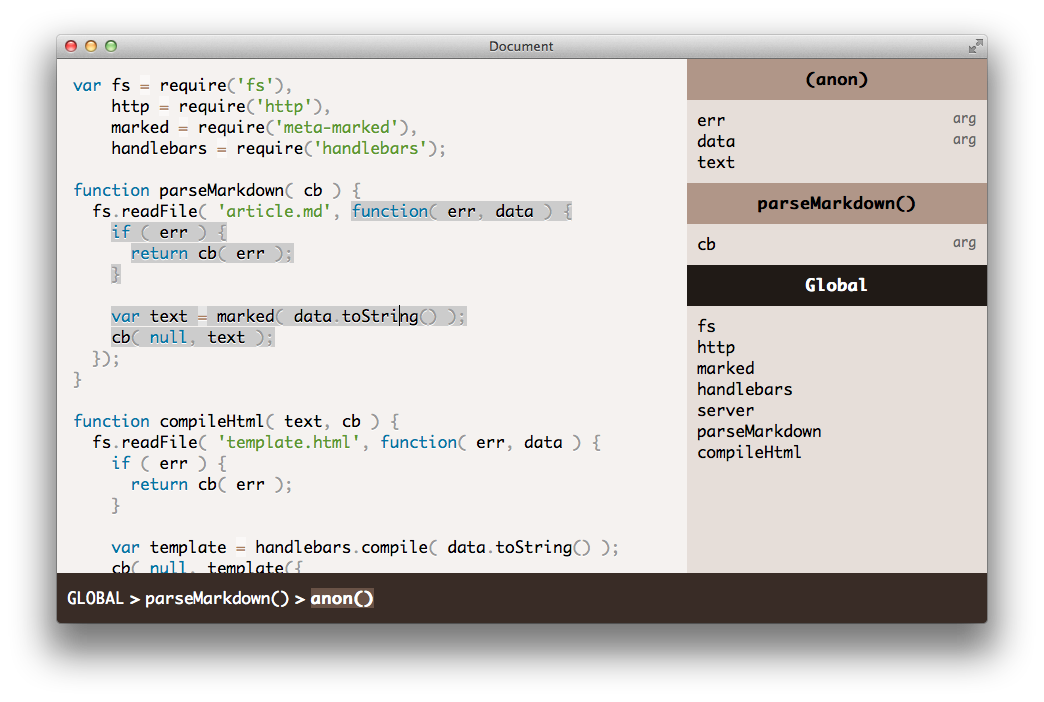
\includegraphics[keepaspectratio,width=0.75\textwidth,height=0.75\textheight]{img/prototype-1.png}
\caption{Screenshot of the static prototype run in a browser}
\label{fig:syntaxhighlighting}
\end{figure}

A code syntax highlighter\footnote{Prism, see \url{http://prismjs.com/}}
was used to turn the subject source code into styled \ac{html} tags, to
make it appear as if it was inside of a real code editor. Applying
syntax highlighting was also necessary to see if the different
highlighting techniques, as sketched out in the previous phase, would
interfere with syntax highlighting.

Furthermore, markers in the form of HTML tags were added to the subject
source code, which made it possible to apply different
styles\footenote{For example text colours, background colours, of font styles.}
to regions of the code. This was later used to realize highlighting of
the \glspl{scope-block}.

Two distinct \ac{ui} elements were added: a sidebar and a bottom bar.
The content of both depends on the \emph{current scope}, i.e. the scope
the cursor is placed in.

For each of the nested \ac{scope-block} that the cursor is positioned in
(beginning from the local scope, going outwards up to the global scope),
the sidebar shows a pane. Each pane contains the scope’s name along with
a list of identifiers defined within that scope. The panes are ordered
ascending by logical distance, i.e. the local scope would be on top, the
next surrounding scope beneath it, and so forth; up to the global scope
on the bottom.

The different panes are hardcoded: all panes exist in the markup of the
prototype at all times and are pre-filled with the relevant data, but
are shown and hidden on demand.

The bottom bar shows a horizontal list of scope names. It makes use of
the \emph{breadcrumbs} \ac{ui}
pattern\footnote{In the Yahoo pattern library: \url{https://developer.yahoo.com/ypatterns/navigation/breadcrumbs.html}}.
Each listed scope, beginning from the global scope on the very left, up
to the local scope on the right, can be highlighted and navigated to by
clicking on its label. By
hovering\footnote{Hovering: Placing the mouse cursor over an element.}
over the label, the user can get a preview of the target scope, as it is
highlighted in the editor alongside the currently active scope.

\subsection{Constraints}\label{constraints}

The static prototype has some drawbacks, some of which might influence
its quality. The most obvious one is the fact that it only works with a
static, predefined source code, which is manually adapted to serve the
prototype’s purpose. This implies that

\begin{enumerate}
\def\labelenumi{\arabic{enumi}.}
\itemsep1pt\parskip0pt\parsep0pt
\item
  changes can not be made to the code, which makes the experience of the
  prototype very different from a real code editor, and
\item
  it is hard to tell if the prototype works similarily well with code
  that is more complex, less complex, or of an overall different style.
\end{enumerate}

The fact that there are no text editing facilities comes with another
drawback, namely the absence of a cursor. If a cursor cannot be placed
anywhere in the editor, the „activation“ of a scope block must be
achieved differently. In the case of this prototype, it is solved by
clicking on a piece of code. However, clicking anywhere in the line
besides the actual text will not change the active scope.

\subsection{Evaluation of the static
prototype}\label{evaluation-of-the-static-prototype}

The prototype was tested with two developers in individual in-person
walkthrough sessions. The users were introduced to the concept, if they
were not familiar with it already, and explained the basic constraints
of the prototype (as mentioned above). They were then able to explore
and test the prototype to their likings. One of the two sessions were
recorded using a screencast.

(screencast von kamil durchhören und ergebnisse hier rein) - besser als
papier, weil dynamisch, „play around“

\section{Final prototype}\label{final-prototype}

The second prototype, which emerged into a final prototype, was built as
a working prototype rather then a proof-of-concept. It was integrated
into the Atom\footnote{See \url{https://atom.io/}} text editor as a
so-called \emph{package}, published as \gls{oss} and was made publicly
available for using and testing.

\subsection{The prototyping platform}\label{the-prototyping-platform}

\begin{itemize}
\itemsep1pt\parskip0pt\parsep0pt
\item
  why is integration into a real ide/editor important?
\end{itemize}

There are different approaches to user testing in the \ac{ucd} process.
Common with the \ac{hci} community is the \emph{lab} approach:
prototypes are tested in isolated environments. However, this is
criticized by \ldots{} and \ldots{}

For the prototype to yield meaningful results, it had to be integrated
into a real \ac{ide} or text editor. This allowed it to be used in a
real-life situation, in the daily development workflows of its users.

As a prototyping platform, the author decided on the Atom text editor.
By the time of writing, Atom is a relatively young project with a
growing community and ecosystem. The reasons for deciding in favour of
Atom are in three characteristics: the technology it is built on, its
internal software architecture, and the user group it is targeting.

Atom is built on web technologies, namely WebKit and Node.js. WebKit is
the browser engine used by Google Chrome and Apple Safari and is
therefore responsible for the \acl{ui} of Atom. Node.js is the
JavaScript platform responsible for running any non-\ac{ui} logic.

Atom is written in
CoffeeScript\footnote{CoffeeScript is a programming language that transcompiles to JavaScript.}

Consequently, Atom packages can be written in CoffeeScript or
JavaScript, using HTML and CSS for the \ac{ui}.

As the author is familiar with these technologies

\begin{itemize}
\item
  text editor by github
\item
  open source
\item
  built in web technology
\item
  both its background, its technologyy and the package ecosystem suggest
  that it is targeted towards web developers, ergo javascript as well
\item
  hackable
\item
  Github \& Atom
\item
  CoffeeScript
\end{itemize}

\subsection{Parsing and gathering relevant
information}\label{parsing-and-gathering-relevant-information}

For the prototype to be as \emph{complete} and \emph{correct} as
possible, it was built on top of an existing JavaScript parser called
Esprima\footnote{See http://esprima.org/}. The process of extracting the
relevant scope structure and annotations from the \ac{ast} will not be
discussed here in greater detail, but is instead described in a blog
post by the author \cite{tvo}.

However, it is important to mention what data structures are extracted
from the source code. Analoguous to the nature of JavaScript scope as
described in chapter \ref{}, the data structure is a hierarchy of
objects. Each object represents a scope and may have metadata as well as
a list of identifiers attached to it. An identifier is either a child
scope (as created by a function) or a variable. For scope objects, the
metadata are its name and its location in the source code (row and
column of the start and end points), whereas for variables the metadata
are its name, location, if it is hoisted, by which identifiers it is
shadowed, and which identifier it is shadowing.

A diagram of an exemplary data structure is shown in the figure
\ref{parser}.

Using this data structure, the prototype can show meaningful data to the
user.

\begin{itemize}
\itemsep1pt\parskip0pt\parsep0pt
\item
  Turn AST into something meaningful
\item
  detect hoisting and shadowing
\end{itemize}

\subsection{Interface and
Interactions}\label{interface-and-interactions}

The design respects that the subject of a developer’s work is the code
itself, not the tools that surround it. This is why the solution
integrates into the most important part of the IDE, the text editor,
directly. The features built into the editor itself will be called
\emph{inline} features.

Atom’s interface is, by default, threefold: the text editor takes the
most space; on its left is a sidebar containing a file browser, and on
the bottom is a status bar. As many web browsers, text editors, and
IDEs, multiple open files are accessed through \emph{tabs} on the top of
the screen. The tabs are important, because the \si will only be active
as long as an editor with a JavaScript file is in the foreground.
Whenever the user switches to another tab, the \si is activated or
deactivated, depending on if the tab contains a JS file or not.

Whenever the \si is active, two things are obvious: on the bottom of the
editor, a panel is shown which we call \emph{bottom bar}, and the
current scope is highlighted inline.

\begin{itemize}
\itemsep1pt\parskip0pt\parsep0pt
\item
  scope inspector inly active when in a javascript file
\end{itemize}

\subsubsection{Inline scope
highlighting}\label{inline-scope-highlighting}

As explained above, the \emph{current scope} is the immediate scope the
cursor is placed in. It is emphasized by highlighting it through a
lighter or darker background colour (depending on Atom’s colour scheme).
If the cursor is placed in a different scope, the formerly active scope
is un-highlighted, and the now active scope is highlighted instead.

While the static prototype implements \emph{exclusive highlighting},
this prototype now implements \emph{inclusive highlighting}, which means
that the inner scope are highlighted as well. This is due to technical
reasons; building exclusive highlighting into the prototype would have
taked a lot more time. In further iterations of the prototype, an option
to enable and disable exclusive highlighting could be provided.

The bottom bar contains a toggle
button\footnote{A switch in the form of a button, which can be either *on* or *off*.}
to enable or disable highlighting of the global scope. Highlighting the
global scope with \emph{inclusive highlighting} is not useful, as the
whole file would be highlighted (and there would be nothing left to
contrast the highlight to).

\subsubsection{Bottom bar}\label{bottom-bar}

The bottom bar serves two purposes: it provides a quick glance of where
in the scope hierarchy the cursor is and provides quick access to two
settings.

On the right side of the bottom bar, to toggle buttons allow for
enabling and disabling of two features. The right button, showing a list
icon, shows or hides the sidebar. The left button with the label
„Highlight Global“ toggles the highlighting of the global scope (as
described above).

The left side of the bottom bar shows the breadcrumbs known from the
static prototype. The breadcrumbs, implemented as simple buttons, are
labeled with the corresponding scope name. The global scope is always on
the left, whereas the currently local, active scope is on the right. By
hovering over any of the breadcrumb buttons, the user can preview the
respective scope highlighting in the editor. The preview is applied in
addition to the currently active highlight in a different colour.

By hovering over the breadcrumbs from left to right or from right to
left, the user can make the relationship between the logical structure
of the JavaScript program (in the form of hierarchic scopes) and the
textual structure (in the form of code) visible.

\subsubsection{Sidebar}\label{sidebar}

The sidebar shows content depending on the currently active scope.
Similarily to the static prototype, the sidebar lists one pane for each
scope in the hierarchy of the active scope. The active scope is listed
on top, while its ancestors are listed below, up to the global scope on
the very bottom.

Each pane is entitled by the name of the scope. In case of function
scope, the name of the function becomes the scope name („(anonymous
function)“ in the case of an unnamed function expression). In case of
the global scope, the name is „GLOBAL“.

Underneath the title, the names of all identifiers defined within the
scope are listed, along with certain attribute annotations.

\begin{itemize}
\itemsep1pt\parskip0pt\parsep0pt
\item
  Function parameters are listed first. They appear with the annotation
  „param“, set in smaller text size to the right.
\item
  General variables follow the parameters. If they are not shadowed,
  they have no annotations.
\item
  Functions are the last entities in the list. They are connotated with
  a pair of parantheses „()“.
\end{itemize}

The listed identifiers show also if they are hoisted, shadowed, or if
they shadow other identifiers. This is indicated by different stylistic
changes.

\begin{itemize}
\itemsep1pt\parskip0pt\parsep0pt
\item
  Hoisted identifiers have a small, upwards-pointed arrow on the left
  side of their label. This indicates that their declaration is
  implicility moved upwards in code.
\item
  Shadowed identifiers are printed in a more subtle text colour. Besides
  that, their label is striked-through to indicate that they are not
  accessible within the given descendant scope.
\item
  Identifiers that shadow other identifiers in ancestor scopes are
  printed in a highlight colour. In case of Atom’s standard \ac{ui}
  theme, this is a bright blue colour.
\end{itemize}

\section{User Testing \& Evaluation}\label{user-testing-evaluation}

The goal of user testing was to collect both qualitative and
quantitative data through different methods. The quantitative data
collection was built into the prototype in form of a connection with
Google Analytics\footnote{A website and app analytics platform.}.

\subsection{Test installment}\label{test-installment}

Atom includes a package management system with an online repository,
called \ac{apm}. This system allows any developer to publish Atom
packages and thus make them available for any Atom user to download and
use. Consequently, this prototype was distributed via \ac{apm}.

The author was collaborating with two full-time developers and one
part-time developer. They agreed to install the package and use it over
the course of one week (full-time developers) or one day (part-time
developer), respectively, integrating it into their usual workflows.

In addition to this directed user test, publishing the prototype via
\ac{apm} made it available to the general public. It was announced on
several social networks, especially targeting existing Atom users, with
the goal of getting users to download and use it. A week after
publishing the prototype, the number of downloads counted ???. This way
of testing „in the wild“ makes it harder to gather feedback, compared to
the method of addressing potential users directly. However, the
analytics mechanism built into the prototype yielded quantitative data
for evaluation.

\subsection{Usage metrics}\label{usage-metrics}

The prototype was built with the option to collect usage metrics using
the Google Analytics service. By default, this option was set to
\emph{off}, as the author opposes the unknown tracking of any data.
However, users were asked to enable tracking in Atom’s \emph{settings}
panel for the Scope Inspector package.

If enabled, the following events are tracked:

\begin{itemize}
\itemsep1pt\parskip0pt\parsep0pt
\item
  The package is enabled/disabled
\item
  The sidebar is shown/hidden
\item
  The user hovers over a scope breadcrumb in the bottom bar and thus
  previews a scope highlighting
\item
  The user clicks on a scope breadcrumb in the bottom bar and thus jumps
  to the beginning of scope, making it the active scope and highlighting
  it
\end{itemize}

Through collecting these events, a claim can be made-{}-to a certain
extent-{}-for how helpful certain features are.

\subsection{Evaluation / Interviews}\label{evaluation-interviews}

\subsubsection{Analytics results /
metrics}\label{analytics-results-metrics}

\subsubsection{Interview with full-time
devs}\label{interview-with-full-time-devs}

\begin{itemize}
\itemsep1pt\parskip0pt\parsep0pt
\item
  alexander slansky: using the sidebar for navigation purposes would be
  doll; zeilennummern wären auch klasse
\end{itemize}
